\subsubsection{UC11.1 - Visualizzazione dei prodotti}
\begin{itemize}
\item \textbf{Attori primari}: utente generico;
\item \textbf{Descrizione}: l'utente può visualizzare un insieme di prodotti raggruppati per categoria accedendo alla relativa PLP\ped{G};
\item \textbf{Scenario Principale}: l'utente visualizza i prodotti appartenenti ad una determinata categoria. Ogni prodotto listato nella PLP\ped{G} deve esporre le seguenti informazioni:
\begin{enumerate}
\item[a.] nome;
\item[b.] immagine;
\item[c.] prezzo;
\end{enumerate}
\item \textbf{Precondizione}: l'utente ha cliccato sulla PLP\ped{G} dedicata alla categoria di prodotti scelta;
\item \textbf{Postcondizione}: l'utente visualizza le informazioni relative ai prodotti listati, con le eventuali operazioni disponibili su ognuno di essi.
\end{itemize}
\subsubsection{UC11.2 - Inserimento nel carrello di un prodotto listato}
\begin{itemize}
\item \textbf{Attori primari}: utente generico;
\item \textbf{Descrizione}: l'utente può inserire un prodotto presente sulla PLP\ped{G} nel carrello, con una quantità selezionata pari ad 1. Per effettuare l'azione è sufficiente cliccare sull'apposito pulsante;
\item \textbf{Scenario Principale}:
\begin{enumerate}
\item[a.] l'utente visualizza i prodotti presenti nella lista corrispondente ad una categoria [UC specifico];
\item[b.] l'utente preme il pulsante per l'inserimento del prodotto desiderato nel carrello.
\end{enumerate}
\item \textbf{Precondizione}: l'utente sta visualizzando la PLP\ped{G} contenente il prodotto desiderato;
\item \textbf{Postcondizione}: l'utente ha inserito nel proprio carrello il prodotto con quantità selezionata pari ad 1.
\end{itemize}
\subsubsection{UC11.3 - Filtraggio dei prodotti}
\begin{itemize}
\item \textbf{Attori primari}: utente generico;
\item \textbf{Descrizione}: l'utente può raffinare la propria ricerca andando a filtrare i prodotti presenti nella PLP\ped{G}. Il parametro utilizzabile per eseguire questa operazione è il prezzo;
\item \textbf{Scenario Principale}:
\begin{enumerate}
\item[a.] l'utente abilita il filtro attraverso l'apposita casella;
\item[b.] l'utente digita il prezzo minimo e il prezzo massimo ai quali è interessato;
\item[c.] l'utente applica il filtro cliccando l'apposito bottone.
\end{enumerate}
\item \textbf{Precondizione}: l'utente sta visualizzando i prodotti in vendita listati nella specifica PLP\ped{G};
\item \textbf{Postcondizione}: l'utente ottiene una nuova pagina in cui può visualizzare solo i prodotti presenti nella PLP\ped{G} corrente e compresi nel range di prezzo specificato.
\end{itemize}
\subsubsection{UC11.4 - Visualizzazione errore nessun risultato filtraggio}
\begin{itemize}
\item \textbf{Attori primari}: utente generico;
\item \textbf{Descrizione}: l'utente visualizza un messaggio di errore che lo informa che il filtraggio dei prodotti effettuato utilizzando i parametri da lui inseriti non ha prodotto nessun risultato.
\item \textbf{Scenario Principale}: l'utente effettua un filtraggio sul catalogo digitale selezionando un range di prezzo nel quale non è presente nessun prodotto;
\item \textbf{Precondizione}: l'utente ha effettuato l'operazione di filtraggio nella corrente PLP\ped{G};
\item \textbf{Postcondizione}: viene visualizzato un messaggio che informa l'utente di non aver trovato prodotti compatibili con quanto stabilito attraverso il range di prezzo.
\end{itemize}
\begin{figure}[H]
\centering
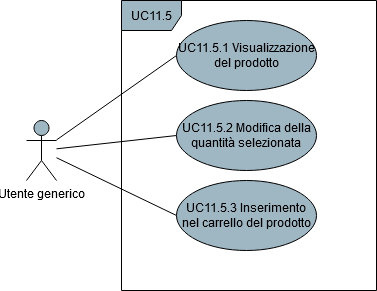
\includegraphics[scale=0.6]{res/UseCase/Immagini/PaginaDelProdotto}
\caption{Diagramma UML per UC11.4 - Pagina del prodotto}
\end{figure}
\subsubsection{UC11.5 - Pagina del prodotto}
\begin{itemize}
\item \textbf{Attori primari}: utente generico;
\item \textbf{Descrizione}: l'utente può accedere ad una pagina per visualizzare tutte le caratteristiche di un prodotto listato. In questa pagina, chiamata anche PDP\ped{G}, è possibile eventualmente aggiungere il prodotto al carrello.
\item \textbf{Scenario Principale}: l'utente clicca sul prodotto da lui desiderato;
\item \textbf{Precondizione}: l'utente si trova in una PLP\ped{G} contenente una lista di prodotti;
\item \textbf{Postcondizione}: l'utente accede alla PDP\ped{G} corrispondente al prodotto desiderato.
\end{itemize}